\documentclass[11pt, a4paper, oneside]{article}

\usepackage{tikz}
\usetikzlibrary{arrows, automata}

\begin{document}
\title{Homework 2}
\author{Aaron Rosen}
\date{Thursday, February 21}
\maketitle

\section*{Problem 1 (Kozen HW2 \#1)}
$\delta(\{s\}, a) = \{s, t\}$\\
$\delta(\{s\}, b) = \{s\}$\\
$\delta(\{s, t\}, a) = \{s, t, u\}$\\
$\delta(\{s, t\}, b) = \{s,\}$\\
$\delta(\{s, t, u\}, a) = \{s, t, u, v\}$\\
$\delta(\{s, t, u\}, b) = \{s\}$\\
$\delta(\{s, t, u, v\}, a) = \{s, t, u, v\}$\\

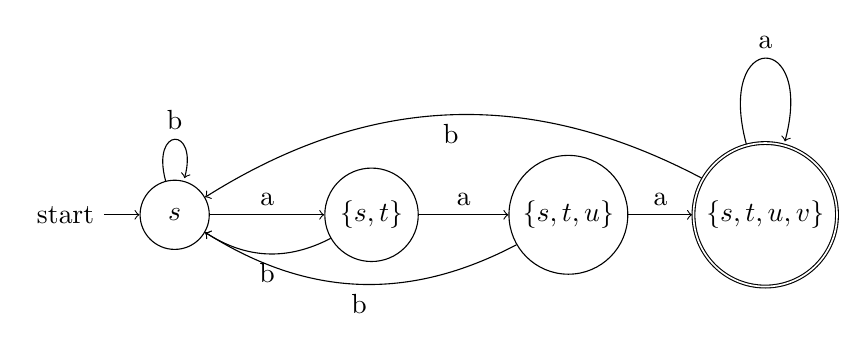
\begin{tikzpicture}[auto, node distance=2.5cm]
	\node[initial, state]   (s)                   {$s$};
	\node[state] 					  (st)   [right of=s]		{$\{s, t\}$};
	\node[state]						(stu)  [right of=st]	{$\{s, t, u\}$};
	\node[state, accepting] (stuv) [right of=stu]	{$\{s, t, u, v\}$};

	\path[->] (s) edge[loop above] node {b} (s);
	\path[->] (s) edge node {a} (st);
	\path[->] (st) edge[bend left] node {b} (s);
	\path[->] (st) edge node {a} (stu);
	\path[->] (stu) edge[bend left] node {b} (s);
	\path[->] (stu) edge node {a} (stuv);
	\path[->] (stuv) edge[loop above] node {a} (stuv);
	\path[->] (stuv) edge[bend right] node {b} (s);
\end{tikzpicture}

\section*{Problem 2 (Kozen HW2 \#2)}
First we define a function $\rho$: RegEx $\rightarrow$ RegEx where\\
$\rho(E) = E$\\  
$\rho(a) = a$\\
Assuming $\rho(\alpha) =$ rev $\alpha$\\
$\rho(\alpha + \beta) =$ rev $\alpha$ + rev $\beta$\\
$\rho(\alpha\beta)=$ rev $\beta$ rev $\alpha$\\
$\rho(\alpha^*) = ($rev$\alpha)^*$\\
\\
Using this definition we can show that if $A\subseteq\Sigma^*$ is regular 
then so is rev $A$\\
\\
We can use $L$: RegEx $\rightarrow P(\Sigma^*)$\\
$L(\rho(E)) = \{E\}$\\
$L(\rho(a)) = \{a\}$\\
$L(\rho(\alpha)) = L($rev$\alpha)$\\
$L(\rho(\alpha + \beta)) = L($rev$\alpha) \cup L($rev$\beta)$\\
$L(\rho(\alpha\beta)) = L($rev$\beta)L($rev$\alpha)$\\
$L(\rho(\alpha^*)) = (L($rev$\alpha))^*$\\
Since we've shown that every regular expression, when reversed is still regular, it follows that the set A of regular expressions will still be regular when reversed.

\section*{Problem 3 (Kozen HW3 \#1)}
\subsection*{(a)}
$(b^*(aa)^*)^*$

\subsection*{(b)}
$(a^*(bb)^*)^*$

\subsection*{(c)}
$(b^*(aa)^*)^* + (a^*(bb)^*)^*b$

\subsection*{(d)}
$((aa)^*(bb)^*)^*b$

\section*{Problem 4 (Kozen HW3 \#2)}
\subsection*{(a)}
NFA\\
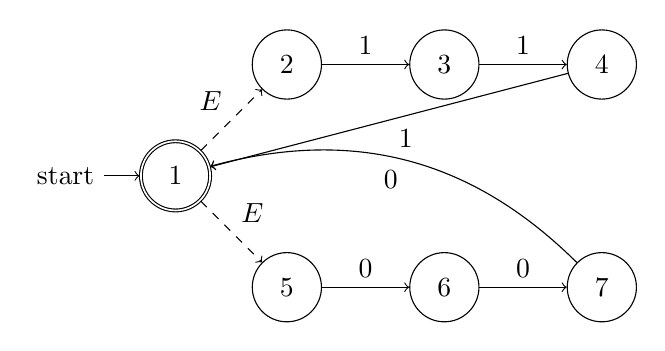
\begin{tikzpicture}[auto, node distance=2cm]
	\node[initial, state, accepting] 	(q1) 	{$1$};
	\node[state] 						(q2) [above right of=q1] {$2$};
	\node[state] 						(q3) [right of=q2] {$3$};
	\node[state] 						(q4) [right of=q3] {$4$};
	\node[state] 						(q5) [below right of=q1] {$5$};
	\node[state] 						(q6) [right of=q5] {$6$};
	\node[state] 						(q7) [right of=q6] {$7$};

	\path[->, dashed] (q1) edge node {$E$} (q2);
	\path[->, dashed] (q1) edge node {$E$} (q5);
	\path[->] 				(q2) edge node {$1$} 			  (q3);
	\path[->] 				(q5) edge node {$0$}				(q6);
	\path[->]				  (q3) edge node {$1$}				(q4);
	\path[->]			    (q6) edge node {$0$}        (q7);
	\path[->]					(q4) edge node {$1$} (q1);
	\path[->]         (q7) edge [bend right] node {$0$} (q1);
\end{tikzpicture}

Delta Function\\
$\Delta(\{1\}, E) = \{2, 5\}$\\
$\Delta(\{2, 5\}, 1) = \{3\}$\\
$\Delta(\{2, 5\}, 0) = \{6\}$\\
$\Delta(\{3\}, 1) = \{4\}$\\
$\Delta(\{6\}, 0) = \{7\}$\\
$\Delta(\{4\}, 1) = \{1\}$\\
$\Delta(\{7\}, 0) = \{1\}$\\

DFA\\
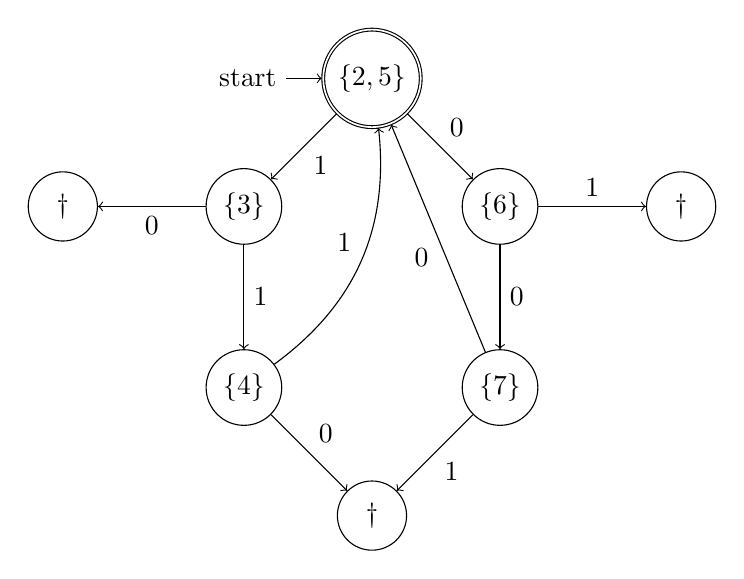
\begin{tikzpicture}[auto, node distance=2.3cm]
	\node[initial, state, accepting] (s25) {$\{2, 5\}$};
	\node[state] (s3) [below left of=s25] {$\{3\}$};
	\node[state] (s4) [below of=s3]  {$\{4\}$};
	\node[state] (s6) [below right of=s25]  {$\{6\}$};
	\node[state] (s7) [below of=s6]  {$\{7\}$};
	\node[state] (dead1) [left of=s3] {$\dagger$};
	\node[state] (dead2) [right of=s6] {$\dagger$};
	\node[state] (dead3) [below right of=s4] {$\dagger$};

	\path[->] (s25) edge node {$1$} (s3);
	\path[->] (s25) edge node {$0$} (s6);
	\path[->] (s3)  edge node {$0$} (dead1);
	\path[->] (s3)  edge node {$1$} (s4);
	\path[->] (s4)  edge node {$0$} (dead3);
	\path[->] (s4) edge[bend right] node {$1$} (s25);
	\path[->] (s6) edge node {$0$} (s7);
	\path[->] (s6) edge node {$1$} (dead2);
	\path[->] (s7) edge node {$1$} (dead3);
	\path[->] (s7) edge node {$0$} (s25);
\end{tikzpicture}

\subsection*{(b)}
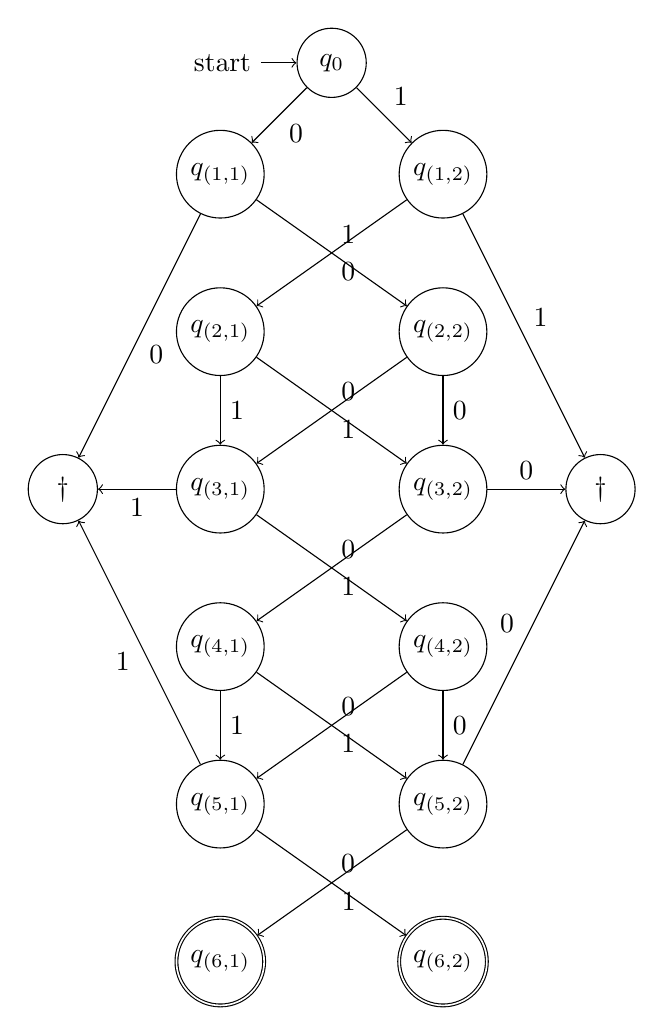
\begin{tikzpicture}[auto, node distance=2cm]
	\node[initial, state] (q0) {$q_0$};
	\node[state] (q11) [below left of=q0]  {$q_{(1,1)}$};
	\node[state] (q12) [below right of=q0] {$q_{(1,2)}$};
	\node[state] (q21) [below of=q11] {$q_{(2,1)}$};
	\node[state] (q22) [below of=q12] {$q_{(2,2)}$};
	\node[state] (q31) [below of=q21] {$q_{(3,1)}$};
	\node[state] (q32) [below of=q22] {$q_{(3,2)}$};
	\node[state] (q41) [below of=q31] {$q_{(4,1)}$};
	\node[state] (q42) [below of=q32] {$q_{(4,2)}$};
	\node[state] (q51) [below of=q41] {$q_{(5,1)}$};
	\node[state] (q52) [below of=q42] {$q_{(5,2)}$};
	\node[state, accepting] (q61) [below of=q51] {$q_{(6,1)}$};
	\node[state, accepting] (q62) [below of=q52] {$q_{(6,2)}$};
	\node[state] (dead1) [left of=q31] {$\dagger$};
	\node[state] (dead2) [right of=q32] {$\dagger$};

	\path[->] (q0) edge node {$0$} (q11);
	\path[->] (q0) edge node {$1$} (q12);
	\path[->] (q11) edge node {$0$} (dead1);
	\path[->] (q11) edge node {$1$} (q22);
	\path[->] (q12) edge node {$0$} (q21);
	\path[->] (q12) edge node {$1$} (dead2);
	\path[->] (q21) edge node {$0$} (q32);
	\path[->] (q21) edge node {$1$} (q31);
	\path[->] (q22) edge node {$0$} (q32);
	\path[->] (q22) edge node {$1$} (q31);
	\path[->] (q31) edge node {$0$} (q42);
	\path[->] (q31) edge node {$1$} (dead1);
	\path[->] (q32) edge node {$0$} (dead2);
	\path[->] (q32) edge node {$1$} (q41);
	\path[->] (q41) edge node {$0$} (q52);
	\path[->] (q41) edge node {$1$} (q51);
	\path[->] (q42) edge node {$0$} (q52);
	\path[->] (q42) edge node {$1$} (q51);
	\path[->] (q51) edge node {$0$} (q62);
	\path[->] (q51) edge node {$1$} (dead1);
	\path[->] (q52) edge node {$0$} (dead2);
	\path[->] (q52) edge node {$1$} (q61);
\end{tikzpicture}

\subsection*{(c)}
NFA\\
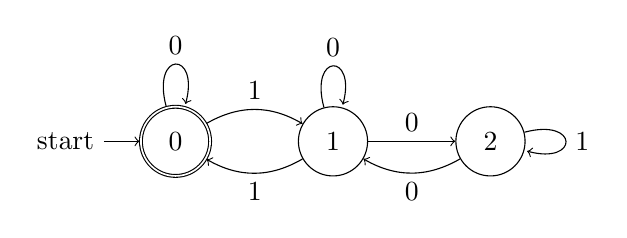
\begin{tikzpicture}[auto, node distance=2cm]
   \node[initial, state, accepting] (q0) {$0$};
   \node[state] (q1) [right of=q0] {$1$};
   \node[state] (q2) [right of=q1] {$2$};

   \path[->] (q0) edge[loop above] node {$0$} (q0);
   \path[->] (q0) edge[bend left]  node {$1$} (q1);
   \path[->] (q1) edge[loop above] node {$0$} (q1);
   \path[->] (q1) edge[bend left]  node {$1$} (q0);
   \path[->] (q1) edge             node {$0$} (q2);
   \path[->] (q2) edge[loop right] node {$1$} (q2);
   \path[->] (q2) edge[bend left]  node {$0$} (q1);
\end{tikzpicture}

Delta Function\\
$\Delta(\{0\}, 0) = \{0\}$\\
$\Delta(\{0\},1) = \{1\}$\\
$\Delta(\{1\}, 0) = \{1,2\}$\\
$\Delta(\{1\}, 1) = \{0\}$\\
$\Delta(\{1,2\}, 0) = \{1,2\}$\\
$\Delta(\{1,2\}, 1) = \{0,2\}$\\
$\Delta(\{0,2\}, 0) = \{0,1\}$\\
$\Delta(\{0,2\}, 1) = \{1,2\}$\\

DFA\\
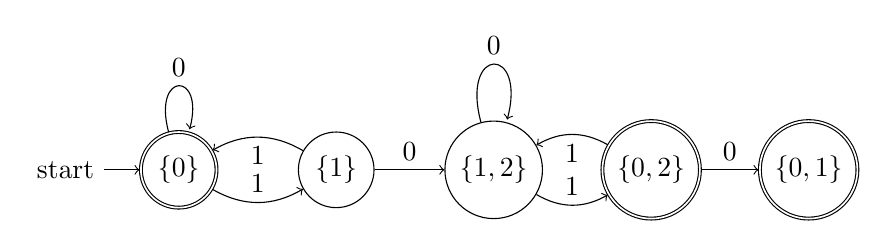
\begin{tikzpicture}[auto, node distance=2cm]
   \node[initial, state, accepting] (q0) {$\{0\}$};
   \node[state]     (q1)  [right of=q0] {$\{1\}$};
   \node[state]     (q12) [right of=q1] {$\{1,2\}$};
   \node[state, accepting] (q02) [right of=q12] {$\{0,2\}$};
   \node[state, accepting] (q01) [right of=q02] {$\{0,1\}$};

   \path[->] (q0) edge[loop above] node {$0$} (q0);
   \path[->] (q0) edge[bend right] node {$1$} (q1);
   \path[->] (q1) edge[bend right] node {$1$} (q0);
   \path[->] (q1) edge node {$0$} (q12);
   \path[->] (q12) edge[loop above] node {$0$} (q12);
   \path[->] (q12) edge[bend right] node {$1$} (q02);
   \path[->] (q02) edge[bend right] node {$1$} (q12);
   \path[->] (q02) edge node {$0$} (q01);
\end{tikzpicture}
\section*{Problem 5 (Kozen HW3 \#3)}
\end{document}
